%Correct the file name.
%X: book number
%Y: part number
%ZZZ: page number in three digits. So page 3 would be 003.

\documentclass[11pt]{amsbook}

\usepackage{../HBSuerDemir}	% ------------------------


\begin{document}

% ++++++++++++++++++++++++++++++++++++++
\hPage{b1p2/469}
% ++++++++++++++++++++++++++++++++++++++
	
	a) $\int x \sqrt{\frac{1+x}{1-x}}dx$ \quad
    	b) $\int^2_0 {\frac{\sqrt{x+1}-1}{\sqrt{x+1}+1}}dx$	
	
	\begin{enumerate}
		

    	\item[81.]
    	Evaluate $\int^b_a \frac{dx} {\sqrt{(x-a)(b-x)}}$

    	\item[82.]
    	If R(x, $\sqrt{ax^2 + bx + c}$ is a rational function of its arguments, show that it becomes a rational function of t upon the substitution: \\
    	a) $ t = \sqrt{a}x+\sqrt{ax^2 + bx + c}$ when $a > 0,$\\
    	b) $ t = \sqrt{(-a).\frac{x - x_1}{x_2 - x}}$ when $a < 0$, where $x_1, x_2$ are the (real) roots of $ax^2+bx+c=0 (x_1 < x_2)$

    	\item[83.]
    	Apply the substitution given in Exercise 82 to transform\\
   	a)$\int\frac{3-\sqrt{4x^2+x-1}}{x+\sqrt{4x^2+x-1}}dx$
    	b)$\int\frac{\sqrt{x - x^2}}{1 + \sqrt{x - x^2}}dx$ \\
    	into ones with integrand as rational function of t.

    	\item[84.]
    	Evaluate $\int \frac{1-\sqrt[3]{x}}{\sqrt{x}}dx$

    	\item[85.]
    	Show that $\int^\pi_0 \frac{x \sin x}{1+\cos ^2x}dx = \frac{\pi^2}{4}$

    	\item[86.]
    	Find the area of the region bounded by the x-axis, the curve $y=xe^{-x}$ and the vertical line through the maximum point.

    	\item[87.]
    	Evaluate $\int x e^x \cos x dx$

    	\item[88.]
    	Find the area between the two curves:\\
    	a)$y=\ln x, y = \ln \frac{1}{x}, 1 < x < e $ \\
    	b)$y=\sin ^2x,y = \sec x, \frac{2\pi}{4} < x < \frac{5\pi}{4}$

    	\item[89.]
    	Given $I_n = \int \cos (n \arctan x)dx$, show that $I_{n+2} + 2I_n + I_{n-2} = \frac{4}{n} \sin (n \arctan x)+c$ 

    	\item[90.]
    	Determine the convergence or divergence, and find the value

	\end{enumerate}

\end{document}  

%==== templates ====

%==== environments ====

%\begin{figure}[htb]
%	\centering
%	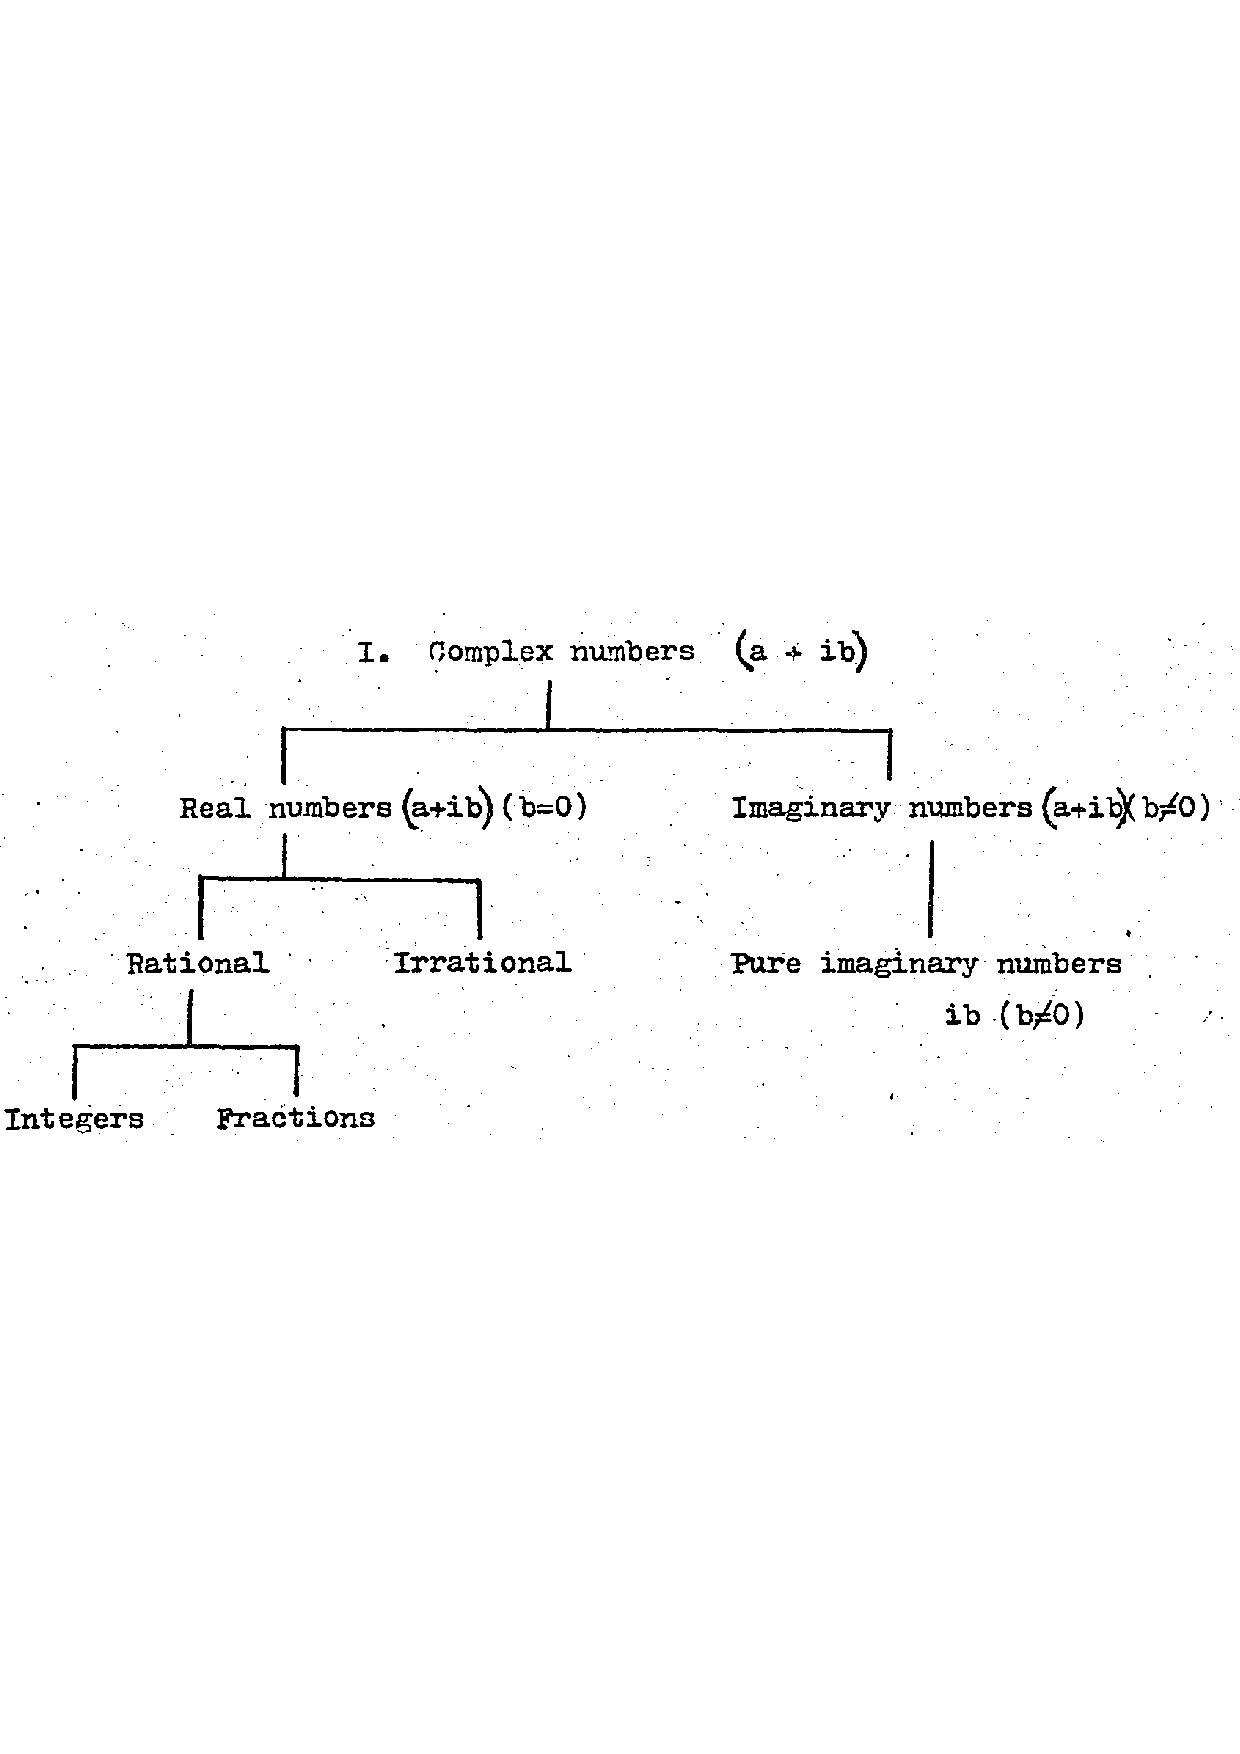
\includegraphics[width=0.9\textwidth]{images/SD-1-1p15A}
%	\caption{Classification of complex numbers}
%	\label{fig:classificationOfComplexNumbersA}
%\end{figure}

%\begin{center}
%\begin{tabular}{cc}
%\end{tabular}
%\end{center}

%\begin{exmp}
%\begin{hSolution}
%\end{hSolution}
%\end{exmp}

%\begin{hEnumerateAlpha}
%\end{hEnumerateAlpha}

%\begin{hEnumerateRoman}
%\end{hEnumerateRoman}

%$
%\begin{bmatrix}
%\end{bmatrix}
%$

%\frac{aaaa}{bbb}
%\frac{a_{n}}{b_{n}}
%\left( aaaa \right)
%\Longrightarrow

%\begin{multicols}{2}
%	bb
%\columnbreak
%	aa
%\end{multicols}
